% !TEX spellcheck = en_US

\documentclass[conference]{IEEEtran}
\usepackage{cite}
\usepackage{amsmath,amssymb,amsfonts}
\usepackage{algorithmic}
\usepackage{graphicx}
\usepackage{textcomp}
\usepackage{xcolor}
% add hyperlinks, delete all .aux files if adding hyperref after previous build
\usepackage{hyperref}
% support for unicode charcters like "é" and "ñ"
\usepackage[T1]{fontenc}
% Provides generic commands \degree, \celsius, \perthousand, \micro and \ohm
\usepackage{gensymb}
% splits a section into multiple columns
\usepackage{multicol}
\def\BibTeX{{\rm B\kern-.05em{\sc i\kern-.025em b}\kern-.08em
    T\kern-.1667em\lower.7ex\hbox{E}\kern-.125emX}}
\begin{document}

\title{Validation of Subhourly Clipping Loss Error Corrections}

\author{\IEEEauthorblockN{Abhishek Parikh\textsuperscript{1}, Kevin Anderson\textsuperscript{2}, Kirsten Perry\textsuperscript{2}, William B. Hobbs\textsuperscript{3}, and Mark A. Mikofski\textsuperscript{1}}
	\IEEEauthorblockA{\textsuperscript{1}DNV, San Diego, CA, 92123, USA }
    \IEEEauthorblockA{\textsuperscript{2}NREL, Golden, CO, 80401, USA }
    \IEEEauthorblockA{\textsuperscript{3}Southern Company, Birmingham, AL, 35203, USA }}

\maketitle

\begin{abstract}
Under-performance of PV systems is an important issue that increases risks for investors. Recently some attention has focused on underestimation of inverter clipping losses as a possible source of over-prediction where sub-hour solar variability is high. Several models and data sets have been analyzed over the past few years, with the aim of quantifying, predicting, and correcting under-predicted clipping loss errors for sites with high DC/AC and solar variability. In this report we compare operational data with a machine learning model developed at NREL to correct hourly weather predictions. In addition, the model is expanded to include site meta-data like DC/AC as factors, so that the model is flexible enough to be used for reducing clipping loss error in energy assessments for a wide variety of sites. \textit{\color{red}add more details about test sites and results here when we have them.}
\end{abstract}

\begin{IEEEkeywords}
inverter, clipping, solar, irradiance, variability, performance, modeling, TMY
\end{IEEEkeywords}

\section{Introduction}
In their "2020 Solar Risk Assessment" \cite{Matsui2020}, kWh Analytics warned that systematic underproduction across the industry exposes investors to increased risk. DNV found that a sample of 39 projects from 2019 were under-performing compared to their pre-construction energy assessments by up to 3\% on average as shown in Fig.~\ref{fig:project-underperformance}. NextEra reported that, "Sub-hour solar resource variability impacts actual energy production by approximately 1-4\%." Cormode, \textit{et al.}, explained that energy assessments based on hourly weather, like typical meteorological year (TMY) data-sets, underestimate inverter clipping losses by up to 5\% for projects with intra-hourly solar variability especially for high DC/AC \cite{Cormode2019}. This is demonstrated in Fig.~\ref{fig:irradiance-and-power}, which shows irradiance and power output at 1-minute and 1-hour resolution in the top and bottom panels respectively. On July 10th there is little intra-hour variability, a mostly clear day, and so hourly and sub-hourly simulations are in close agreement. In contrast, July 13th has much higher solar variability, but no clipping is observed in the 1-hour output. However, the 1-minute resolution shows intermittent clipping all day long, indicating that not all of the available irradiance is used by the system, and the hourly simulation underestimates inverter clipping \cite{Kharait}.

\begin{figure}[htbp]
\centerline{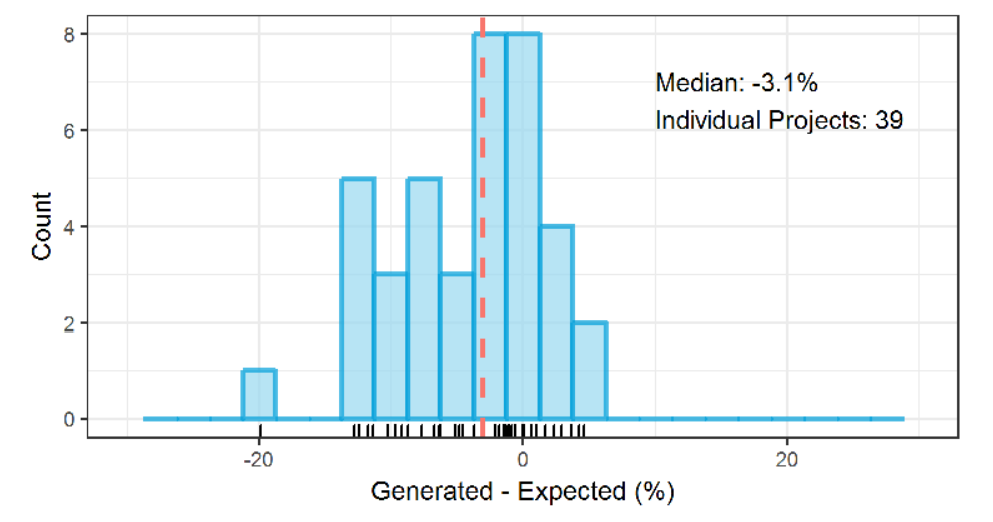
\includegraphics[width=9cm]{fig1.png}}
\caption{Project-average validation results for solar energy assessments. Each project-year was adjusted for interannual variability by scaling production by the ratio of TGY to historical monthly insolation.}
\label{fig:project-underperformance}
\end{figure}


\begin{figure}[htbp]
\centerline{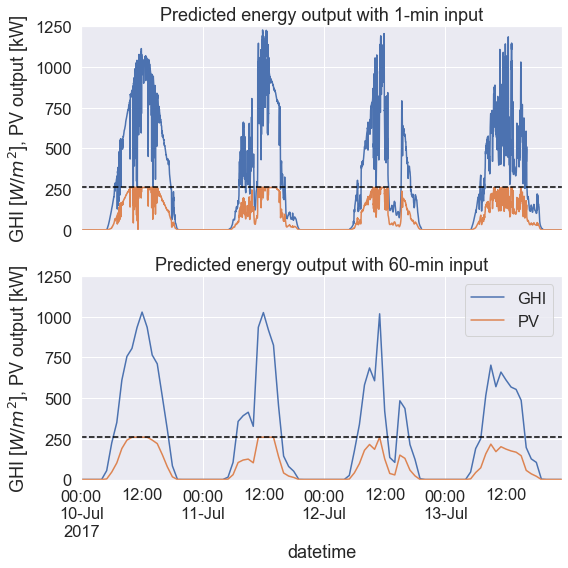
\includegraphics[width=9cm]{hourly_v_1-min_clipping.png}}
\caption{Irradiance input from the NIST test-bed weather station in Gaithersburg, MD, and predicted energy output using SolarFarmer at time-resolution of 1-minute, \textit{top panel}, and 1-hour, \textit{bottom panel}. The black dashed line in both panels shows the inverter rated power, 260-kW.}
\label{fig:irradiance-and-power}
\end{figure}

Several methods have been proposed to correct clipping loss errors in hourly predictions \cite{Cormode2019,Kharait,Anderson2020,Bradford}, but only NextEra validated their method with operational data \cite{Bradford}. In this report, we adopt the NREL machine-learning based model \cite{Anderson2020} to predict clipping loss corrections and apply them to hourly energy assessments. The adjusted energy assessment is then validated against operational data from the same site, and we report on the average and distribution of validation errors. \textit{\color{red}add some results here when we have them.} We have obtained data from seven operating PV systems in different climates and with a range of DC/AC. In this paper we will present the first of these systems, outline our method, and present preliminary results. The final paper will present validation results from all seven sites plus the NIST ground array \cite{Boyd2017b} as a benchmark.

\section{Methods}

\subsection{Model}

The machine-learning model developed at NREL has already been described in detail \cite{Anderson2020}. \textit{\color{red}Kirsten and Kevin, please fill in details here.} The model currently has been trained on a fixed layout with a single DC/AC. In this report, DC/AC has been introduced as a new continuous factor, and the model has been retrained with a range of DC/AC to allow it to be used to correct clipping loss errors for a wide range of common project configurations. As described in \cite{Anderson2020}, the model has been trained using high quality irradiance measurements from SURFRAD \cite{Augustine2000} and 1-minute to 30-minute clipping loss errors predicted using SAM \cite{Freeman2018}. The resulting trained model is then used to make predictions at the operational sites.

\textit{\color{red}Image of flow chart?.}

\subsection{Validation}
A challenge in validating the clipping loss correction model is the lack of quality high-frequency irradiance measurements that are co-located with operational PV systems. Therefore this model differs from traditional approaches for model training and validation because it relies on SURFRAD measurements and SAM simulated data to train the model, but uses operational data from different sites for validation. So no holdout methods are required in validating this model because the training and validation data sets are already independent. The downside of this method is that any systematic biases in SAM are baked into the clipping loss correction model. In future work, if a large population of high-frequency irradiance and co-located operational data are obtained, the model can be retrained holding out a subset of the data for validation. This procedure would have the benefit of incorporating any physical effects that are not captured by SAM.

Before the operational data is used in validation, it is reviewed to remove any outliers that could disrupt the validation. \textit{\color{red}Abhi can you please discuss some of the methods you used to clean the data, and explain how you identified outliers and why you removed them. Please also explain if you use only a subset of inverters or only a particular period of time, why you chose them and how. Discuss any caveats either here, in the results, or in the conclusions.}

Several metrics are used to measure the reduction in clipping loss errors from the hourly energy assessment, and identify if there are any unknown factors that are systematically affecting the results.

\begin{itemize}
\item \textbf{bias}: delta between the corrected energy assessment predictions and the measured operational data, so positive bias means over-predicted energy output 
\begin{equation}
\Delta E={E_\text{predicted}} - {E_\text{measured}}\label{eq:bias}
\end{equation}
Where $E$ is the energy output.
\item \textbf{mean bias error (MBE)}: average of the bias, beware a low MBE might hide seasonal or diurnal bias
\begin{equation}
\mathit{MBE}=\frac{\sum_{n=1}^N{\Delta_n}}{N}\label{eq:mbe}
\end{equation}
Where $n$ is a single timestep, and $N$ is the total period of time. For example, with hourly timesteps, $N=8760\text{[hrs]}$, the number of timesteps in a typical annual energy assessment.
\item \textbf{root mean squared error}: squares of the bias are positive, removing any cancellation of opposing errors, and therefore gives a measure of the width of the error distribution
\begin{equation}
\mathit{RMSE}=\sqrt{\frac{\sum_{n=1}^N{\Delta_n^2}}{N}}\label{eq:rmse}
\end{equation}
\item \textbf{mean absolute error (MAE)}: a measure of the average bias that removes any cancellation of opposing errors
\begin{equation}
\mathit{MAE}=\frac{\sum_{n=1}^N{\left|\Delta_n\right|}}{N}\label{eq:mae}
\end{equation}
\item \textbf{error distribution}: a histogram of the bias should look like a normal distribution, centered at zero
\item \textbf{temporal correlation}: a plot of the bias aggregated monthly or by hour of the day should have a uniform flat distribution
\item \textbf{auto-correlation}: a plot of the bias versus dependent parameter, energy output ($E$) should also have a uniform distribution
\item \textbf{cross-correlation}: plots of the bias versus independent parameters like irradiance, DC/AC ratio, clearness index, \textit{etc.}, should all have a uniform distributions
\end{itemize}


\section{Results}

\subsection{Model Parameters}

\textit{\color{red}a few tables of the inputs for SAM and the ML model and the parameters that were derived from the training data.}

\begin{table}[htbp]
\caption{Table Type Styles}
\begin{center}
\begin{tabular}{|c|c|c|c|}
\hline
\textbf{Table}&\multicolumn{3}{|c|}{\textbf{Table Column Head}} \\
\cline{2-4} 
\textbf{Head} & \textbf{\textit{Table column subhead}}& \textbf{\textit{Subhead}}& \textbf{\textit{Subhead}} \\
\hline
copy& More table copy$^{\mathrm{a}}$& &  \\
\hline
\multicolumn{4}{l}{$^{\mathrm{a}}$Sample of a Table footnote.}
\end{tabular}
\label{tab1}
\end{center}
\end{table}

\subsection{Validation Metrics}

\textit{\color{red}a few tables and figures about site A operational performance. And of course! the metrics discussed above. Definitely show a histogram of the bias, a plot of the bias vs. output, and a table of the MBE, MAE, \& RMSE. Then definitely a discussion of the results. Are they good, okay, why do we think so? what assumptions are there that could be affecting the outcomes?}

\section{Conclusions}
Improvements in prediction of PV system performance increases investor confidence. Over-prediction occurs in typical energy assessments that use hourly data if the sites have sub-hourly solar variability and high DC/AC because clipping losses are underestimated. These errors have been quantified using a machine-learning model trained on high-frequency solar irradiance data and simulated operational data to create clipping loss error corrections. The corrections were applied to a typical hourly energy assessment of an existing operational site and compared to the measured output from the same site. The mean bias error was reduced from X\% to Y\% per year. The final report will report the validation results for an additional 7 operating PV sites. with the goal of providing a standard method for correcting clipping loss errors from typical energy assessments, and therefore decreasing investor risk.

\section*{Acknowledgment}

Acknowledge the data providers if they want it? Anything for Southern Company or DNV?

This work was authored by Alliance for Sustainable Energy, LLC, the manager and operator of the National Renewable Energy Laboratory for the U.S. Department of Energy (DOE) under Contract No. \textit{\color{red}is this needed?}. Funding provided by the U.S. Department of Energy’s Office of Energy Efficiency and Renewable Energy (EERE) under Solar Energy Technologies Office (SETO) Agreement Numbers \textit{\color{red}is this needed?}. The views expressed in the article do not necessarily represent the views of the DOE or the U.S. Government. The U.S. Government retains and the publisher, by accepting the article for publication, acknowledges that the U.S. Government retains a nonexclusive, paid-up, irrevocable, worldwide license to publish or reproduce the published form of this work, or allow others to do so, for U.S. Government purposes.

\bibliographystyle{IEEEtran}
% argument is your BibTeX string definitions and bibliography database(s)
\bibliography{IEEEabrv,bibliography}

\end{document}
